\documentclass{IEEEtran}

\usepackage{cite}
\usepackage{amsmath}
\usepackage{amssymb}
\usepackage{url}
\usepackage{graphicx}
\usepackage{booktabs}
\usepackage{microtype}
\usepackage[table]{xcolor}
\usepackage{tikz}
\usetikzlibrary{positioning,arrows.meta,fit,backgrounds}
\usepackage[hidelinks]{hyperref}

\definecolor{phase1blue}{RGB}{52,152,219}
\definecolor{phase2green}{RGB}{46,204,113}
\definecolor{phase3orange}{RGB}{230,126,34}
\definecolor{phase4purple}{RGB}{155,89,182}

\title{{\LARGE\textbf{Fairness-Aware Routing in Quantum Networks \& Clinical Settings}}\\
{\Large\textit{via Multi-Armed, Contextual, and Informative Bandit Methods}}\\
{\large\texttt{(Approach Writeup)}}}

\author{%
\begin{minipage}{0.48\textwidth}
\begin{center}
{\bf Piter Z. Garcia}\\
\begin{small}
MS Data Science / Decision-Making \& Algorithmic Fairness\\
Rochester Institute of Technology (RIT)\\
{\it pizg8794@g.rit.edu}
\end{small}
\end{center}
\end{minipage}
\hfill
\begin{minipage}{0.48\textwidth}
\begin{center}
{\bf Dr. Daniel Krutz, Travis Desell}\\
\begin{small}
Department of Software Engineering, Data Science\\
RIT Research Advisors\\
{\it dxkvse@g.rit.edu, tjdvse@g.rit.edu}
\end{small}
\end{center}
\end{minipage}%
}

\begin{document}
\maketitle

%% ─────────────────────────────────────────────────────────────
\section{Approach Overview}
%% ─────────────────────────────────────────────────────────────

Quantum-network routing and clinical resource allocation are, at their
core, \textit{routing problems}---and both fail for the same reason:
\textit{missing context}. In quantum networking, entanglement and qubit
resources must be routed across competing flows under probabilistic link
success and scarcity; standard policies underperform because they ignore,
misuse, or lose the context that would guide fair allocation. In clinical
settings, diagnostic and treatment resources are routed among patients under
uncertainty and partial information; tools calibrated on non-representative
populations are blind to the context of those they exclude. 
In both cases, the groups whose context is missing absorb the worst outcomes---and the
degradation is a direct performance failure. This shared root cause makes the two
domains structurally comparable and motivates a unified evaluation framework.

The contribution is a reproducible bandit-method framework spanning three
context-richness levels---non-contextual MABs, contextual CMABs, and
informative iCMABs---designed specifically to probe what happens when context
is absent, partially available, or actively recovered. Two prior works anchor
the testbeds: equitable bioinformatics work provides the clinical fairness
foundation \cite{garcia2025equitable_bioinformatics}, and threat-aware
quantum routing work provides the network environment
\cite{garcia2026threat_aware_quantum_routing}. Quantum networking is an
emerging technology with growing practical relevance for communication and
resource allocation; pairing it with clinical fairness through the structural
bridge of missing-context routing positions this work at the intersection of
present need and future-oriented system design.

%% ─────────────────────────────────────────────────────────────
\section{Motivating Workflows}
%% ─────────────────────────────────────────────────────────────

\subsection{Clinical Routing Workflow}
The clinical decision-maker routes resources---screens, confirmatory tests,
escalation follow-ups---among patients under incomplete, delayed, or
group-unequal context. As demonstrated in the COVID-19 response, uneven
routing context systematically under-resources certain subgroups, producing
higher false-negative rates, delayed escalation, and inferior care. A
compounding failure reveals a second dimension: diagnostic protocols built
from non-representative control groups calibrated thresholds against an
incomplete population, rendering certain groups structurally invisible to the instrument. 
The result is missing context at the point of decision, amplifying risk for the very groups already
bearing the highest burden.

\subsection{Quantum Routing Workflow}
The quantum decision-maker routes entanglement by selecting paths and
allocating scarce entanglement-generation attempts among competing flows
under noisy, stale, or partial context. Standard MABs ignore context
entirely; CMABs use it but remain vulnerable to noise and missingness.
Empirical testing reveals that iCMABs consistently outperform both---because
they recover and correctly weight context the other methods miss or misuse.
This is the same structural problem. Missing context
in the routing policy produces the same outcome as in the clinical instrument: 
the groups whose information is least represented absorb the worst outcomes.

%% ─────────────────────────────────────────────────────────────
\section{Shared Domain Model}
%% ─────────────────────────────────────────────────────────────

The shared domain model (Figure~\ref{fig:domain_model}(a)) organizes the
routing-decision process into four phases---
\textcolor{phase1blue}{\textbf{Environment}} (blue),
\textcolor{phase2green}{\textbf{Context Observation}} (green),
\textcolor{phase3orange}{\textbf{Routing Decision}} (orange),
\textcolor{phase4purple}{\textbf{Evaluation and Mitigation}} (purple)---
structurally identical across testbeds. Operational semantics differ:
a routing action is a diagnostic decision in the clinical domain and a
path-selection decision in the quantum domain; fairness is measured as
outcome disparity across patient or network flow groups.

The COVID-19 pandemic provides a clear real-world example of this routing
problem in practice. Diagnostic tests were scarce, unevenly routed, and delayed, 
producing measurably worse outcomes for Black, Latino, and other minority 
groups---confirming that unfair routing is a performance failure, not only an equity concern.

What unifies this framework at a deeper level is that both domains share
not only the routing structure, but the root cause of failure: missing
context. In clinical settings, excluded populations are invisible to the
instrument. In quantum routing, iCMABs outperform MABs and CMABs not due to
complexity, but because they recover context the other methods discard. The
underperforming groups in both cases are those whose context was never
properly captured. \textit{Phase~2 is therefore where the root cause of routing 
unfairness lives}---and the primary phase this framework is designed to interrogate. 
\textit{Phase~4}, operationally expanded in Figure~\ref{fig:domain_model}(b),
then detects, logs, and mitigates the downstream consequences before they compound.

%% ─────────────────────────────────────────────────────────────
\section{Design Rationale and Novelty}
%% ─────────────────────────────────────────────────────────────

\subsection{Why This Approach}
To our knowledge, prior work has not evaluated fairness-aware sequential
routing under a unified bandit framework spanning clinical and quantum
domains, nor identified missing context as the shared structural root cause
of routing unfairness across both domains. Clinical bandit research optimizes
treatment decisions without examining how missing population context degrades
routing equity; quantum routing research maximizes throughput without
connecting context missingness to service-equity disparities. Studying them
together produces findings that improve today's clinical systems and inform
routing in tomorrow's quantum-enabled infrastructures where fairness is itself
a performance criterion.

\subsection{Why This Approach Is Stronger Than Simpler Alternatives}
Single-domain approaches cannot verify whether missing context drives routing
unfairness structurally or only situationally; findings remain confined to
one state space and one fairness definition. Post-hoc audits cannot capture
how context gaps compound into routing disparities over time under learning.
This framework measures fairness at every step under the same partial-feedback
conditions that make routing difficult in practice, enabling real-time
detection of where and when missing context causes disparity, and direct
comparison of policies that ignore, use, or recover that context.

\subsection{Design and Implementation Decisions Made}
\textit{Bandits over full RL:} both domains return only partial feedback,
making bandit methods the correct formulation. \textit{Simulation-first
clinical testbed:} it allows controlled injection of missing context,
noise, and group-specific degradation without sensitive patient data.
\textit{Existing quantum environment extended:} reusing a grounded,
threat-aware routing environment preserves the domain-realistic missing-context
conditions empirically observed in iCMAB performance. \textit{MAB / CMAB /
iCMAB spectrum:} each level directly operationalizes the core
question---\textit{does recovering missing routing context reduce disparities, or are
additional fairness mechanisms still required?}

\subsection{Connecting Decisions to the Domain Model}
Each design decision maps directly to a phase in
Figure~\ref{fig:domain_model}(a), determining what that phase must do and why.

\textsc{Phase~1 (Environment)} is shaped by the simulation-first clinical
testbed and the quantum environment extension. The simulation introduces
missing and group-unequal context as a controlled variable, making
\textsc{Phase~1} a research instrument, not just a data source. The
quantum extension means \textsc{Phase~1} inherits domain-realistic
conditions---link success rates, entanglement scarcity, threat
signals---thereby reproducing the same missing-context failure mode without adding a new testbed.

\textsc{Phase~2 (Context Observation)} is shaped by the MAB/CMAB/iCMAB
spectrum. Each level defines how much context reaches the policy: none,
structured but potentially incomplete, or actively recovered despite noise
and missingness. \textsc{Phase~2} is the experimental variable and the locus
of the root cause; spanning three levels directly measures how much routing
disparity is explained by missing context alone.

\textsc{Phase~3 (Routing Decision)} is shaped by the bandit choice. Because
both environments return only the outcome of the chosen route---never the
counterfactual---the policy must be a bandit policy. Full RL would require
transition-model information that does not exist. The bandit formulation is
the only structurally honest choice given what \textsc{Phase~4} can return.

\textsc{Phase~4 (Evaluation and Mitigation)} justifies the entire design.
Logging utility and fairness at every step produces a per-step disparity
trajectory, making it possible to pinpoint exactly when missing context
causes disparities to emerge, persist, or resolve under mitigation. The
domain model in Figure~\ref{fig:domain_model}(a) is the organizational
structure that determined every design choice from \textsc{Phase~1} through
\textsc{Phase~4}.

%% ─────────────────────────────────────────────────────────────
\section{Implementation and Evaluation Plan}
%% ─────────────────────────────────────────────────────────────

Both testbeds expose the same policy interface and are driven by the modular
six-layer pipeline shown in Figure~\ref{fig:domain_model}(b), so MAB, CMAB,
and iCMAB methods are evaluated under a shared logging and analysis pipeline.
The clinical simulation models test ordering, retesting, and escalation under
deliberately introduced missing and group-unequal context; the quantum
environment reproduces the domain-realistic context missingness that drives
the empirically observed iCMAB advantage. The reward layer tracks accuracy,
cost, success rate, and latency; the fairness layer tracks clinical
false-negative and delayed-escalation gaps and quantum service-equity gaps
across flow groups. Experiments use explicit configurations, fixed random
seeds, and per-step metric logging; at least one fairness mitigation
mechanism is evaluated to enable comparison among policies that ignore,
partially use, or actively recover missing context.

%% ─────────────────────────────────────────────────────────────
\section{Research Contribution}
%% ─────────────────────────────────────────────────────────────

This work makes three contributions. First, it identifies routing and missing
context as the shared structural ground between clinical and quantum domains,
and constructs a unified fairness-aware sequential decision framework---
visualized in Figure~\ref{fig:domain_model}---for evaluating both under
comparable conditions. Second, it provides a systematic MAB/CMAB/iCMAB
comparison with respect to routing fairness, directly measuring how much
disparity is explained by missing context and how much requires additional
mitigation. Third, by connecting a domain of immediate human health impact to
an emerging technology through their shared missing-context failure mode, the
findings serve both as an evaluation of current systems and a foundation for
next-generation quantum-enabled infrastructures, where fair and
high-performing routing are understood as the same problem.

\begin{thebibliography}{9}\setlength{\itemsep}{0em}
\bibitem{garcia2025equitable_bioinformatics}
Garcia, P.~Z. Equitable Bioinformatics: Enhancing Diagnostic
Decision-Making through {RNA} and Biomarker Data. Course paper
(ISTE~780 Phase~4), Rochester Institute of Technology, 2025.
\bibitem{garcia2026threat_aware_quantum_routing}
Garcia, P.~Z. Threat-Aware Evaluation of Quantum Entanglement Routing
and Qubit Allocation via Hybrid Contextual Bandits. Unpublished
manuscript, Rochester Institute of Technology, 2026.
\end{thebibliography}

%% ─── Figure at end — does not count toward two-page limit ───
\clearpage
\begin{figure*}[!t]
\centering
\resizebox{0.97\textwidth}{!}{%
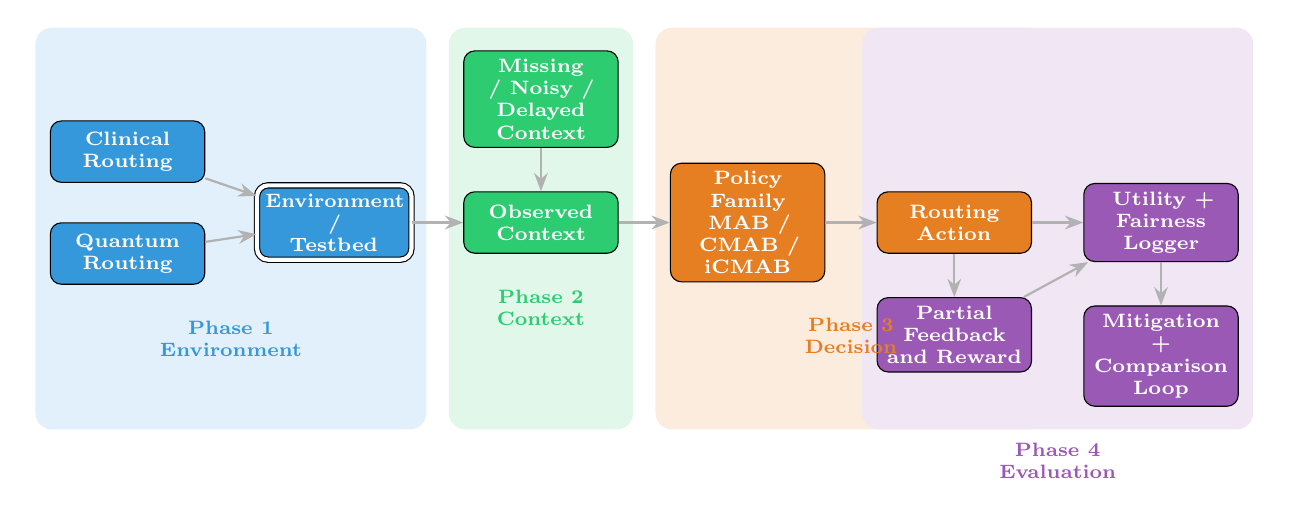
\begin{tikzpicture}[
  font=\scriptsize,
  box/.style={draw, rounded corners=4pt, align=center,
              text width=1.75cm, minimum height=0.78cm,
              inner sep=3pt, text=white, font=\scriptsize\bfseries},
  phase1/.style={box, fill=phase1blue},
  phase2/.style={box, fill=phase2green},
  phase3/.style={box, fill=phase3orange},
  phase4/.style={box, fill=phase4purple},
  arr/.style={-Stealth, thick, gray!60},
  lbl/.style={font=\scriptsize\bfseries, align=center}
]
\node[phase1] (clin)  {Clinical\\Routing};
\node[phase1, below=0.5cm of clin]  (quant) {Quantum\\Routing};
%% double border marks this as the zoomed node
\node[phase1, right=0.65cm of clin, yshift=-0.9cm,
      double, double distance=1.5pt] (env) {Environment /\\Testbed};
\node[phase2, right=0.65cm of env]  (ctx) {Observed\\Context};
\node[phase2, above=0.55cm of ctx]  (deg) {Missing / Noisy /\\Delayed Context};
\node[phase3, right=0.65cm of ctx]  (pol) {Policy Family\\MAB / CMAB / iCMAB};
\node[phase3, right=0.65cm of pol]  (act) {Routing\\Action};
\node[phase4, below=0.55cm of act]  (fb)  {Partial Feedback\\and Reward};
\node[phase4, right=0.65cm of act]  (log) {Utility + Fairness\\Logger};
\node[phase4, below=0.55cm of log]  (mit) {Mitigation +\\Comparison Loop};

\draw[arr] (clin)--(env); \draw[arr] (quant)--(env);
\draw[arr] (env)--(ctx);  \draw[arr] (deg)--(ctx);
\draw[arr] (ctx)--(pol);  \draw[arr] (pol)--(act);
\draw[arr] (act)--(fb);   \draw[arr] (act)--(log);
\draw[arr] (fb)--(log);   \draw[arr] (log)--(mit);

\begin{pgfonlayer}{background}
  \node[inner sep=8pt,
        fit=(clin)(quant)(env)(ctx)(deg)(pol)(act)(fb)(log)(mit)] (all) {};
  \node[inner sep=5pt, fit=(clin)(quant)(env)] (bg1) {};
  \node[inner sep=5pt, fit=(ctx)(deg)]         (bg2) {};
  \node[inner sep=5pt, fit=(pol)(act)]         (bg3) {};
  \node[inner sep=5pt, fit=(fb)(log)(mit)]     (bg4) {};
  \fill[phase1blue!15,   rounded corners=6pt]
      (bg1.west |- all.north) rectangle (bg1.east |- all.south);
  \fill[phase2green!15,  rounded corners=6pt]
      (bg2.west |- all.north) rectangle (bg2.east |- all.south);
  \fill[phase3orange!15, rounded corners=6pt]
      (bg3.west |- all.north) rectangle (bg3.east |- all.south);
  \fill[phase4purple!15, rounded corners=6pt]
      (bg4.west |- all.north) rectangle (bg4.east |- all.south);
\end{pgfonlayer}

\node[lbl, text=phase1blue,   below=0.15cm of bg1] {\textbf{Phase 1}\\Environment};
\node[lbl, text=phase2green,  below=0.15cm of bg2] {\textbf{Phase 2}\\Context};
\node[lbl, text=phase3orange, below=0.15cm of bg3] {\textbf{Phase 3}\\Decision};
\node[lbl, text=phase4purple, below=0.15cm of bg4] {\textbf{Phase 4}\\Evaluation};
\end{tikzpicture}%
}

\vspace{0.2em}
{\small\textbf{(a)} Shared domain model.}
\vspace{0.5em}

%% ── Zoom-in bridge arrow ──────────────────────────────────────
\noindent\hspace{0.03\textwidth}%
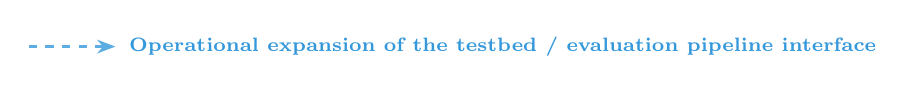
\begin{tikzpicture}[baseline=-0.5ex, font=\scriptsize]
  \draw[-Stealth, thick, phase1blue!80, dashed] (0,0) -- (1.1,0);
  \node[right=1.15cm, font=\scriptsize\bfseries, text=phase1blue]
    at (0,0) {Operational expansion of the \textbf{testbed / evaluation pipeline interface}};
\end{tikzpicture}
\vspace{0.4em}

%% ── (b) Pipeline zoom-in — horizontal, phase1blue!15 background ──
\resizebox{0.97\textwidth}{!}{%
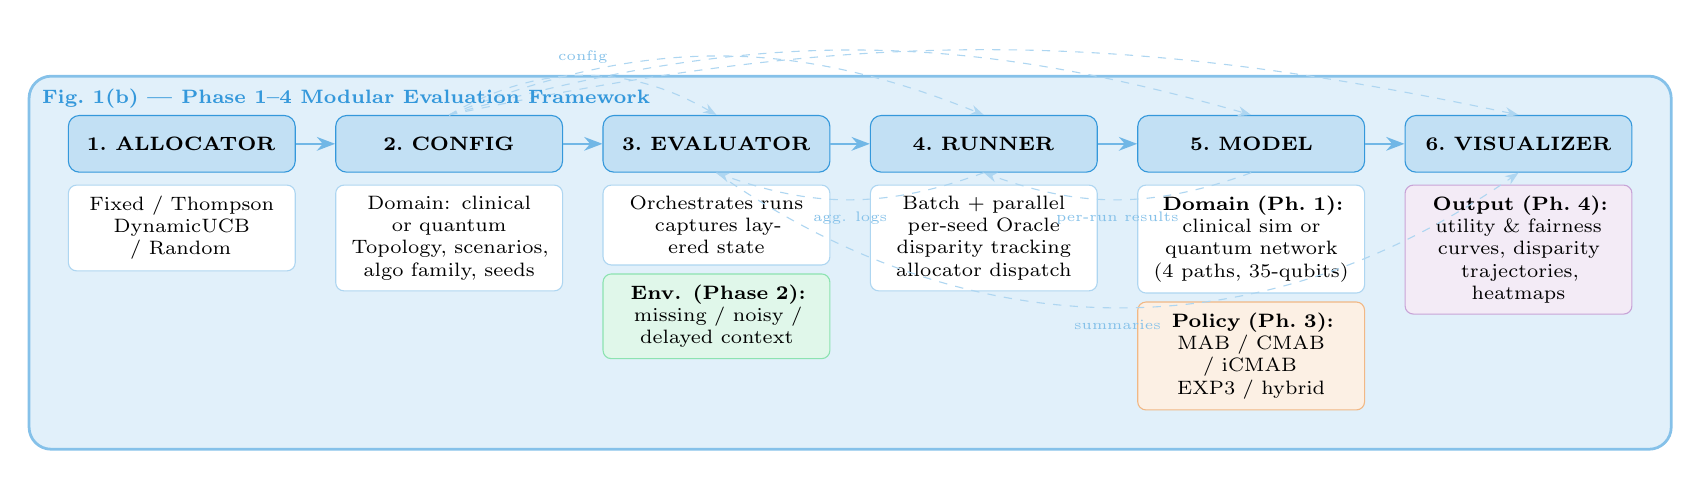
\begin{tikzpicture}[
  font=\scriptsize,
  mod/.style={rectangle, draw=phase1blue, rounded corners=4pt, align=center,
              text width=2.6cm, minimum height=0.72cm,
              inner sep=4pt, font=\scriptsize\bfseries,
              fill=phase1blue!30},
  det/.style={rectangle, draw=phase1blue!40, rounded corners=3pt, align=center,
              text width=2.6cm, inner sep=4pt, font=\scriptsize, fill=white},
  det2/.style={det, fill=phase2green!15,  draw=phase2green!55},
  det3/.style={det, fill=phase3orange!12, draw=phase3orange!55},
  det4/.style={det, fill=phase4purple!12, draw=phase4purple!55},
  arr/.style={-Stealth, thick, phase1blue!70},
  darr/.style={-Stealth, dashed, phase1blue!40},
  lbl/.style={font=\tiny, align=center, text=phase1blue!60}
]

\node[mod] (A) {1.~ALLOCATOR};
\node[det, below=0.15cm of A] (Ad)
  {Fixed / Thompson\\DynamicUCB / Random};

\node[mod, right=0.5cm of A] (C) {2.~CONFIG};
\node[det, below=0.15cm of C] (Cd)
  {Domain: clinical\\or quantum\\Topology, scenarios,\\algo family, seeds};

\node[mod, right=0.5cm of C] (E) {3.~EVALUATOR};
\node[det, below=0.15cm of E] (Ed)
  {Orchestrates runs\\captures layered state};
\node[det2, below=0.1cm of Ed] (Env)
  {\textbf{Env. (Phase~2):}\\missing / noisy /\\delayed context};

\node[mod, right=0.5cm of E] (R) {4.~RUNNER};
\node[det, below=0.15cm of R] (Rd)
  {Batch + parallel\\per-seed Oracle\\disparity tracking\\allocator dispatch};

\node[mod, right=0.5cm of R] (M) {5.~MODEL};
\node[det, below=0.15cm of M] (Md)
  {\textbf{Domain (Ph.~1):}\\clinical sim or\\quantum network\\(4 paths, 35-qubits)};
\node[det3, below=0.1cm of Md] (Alg)
  {\textbf{Policy (Ph.~3):}\\MAB / CMAB / iCMAB\\EXP3 / hybrid};

\node[mod, right=0.5cm of M] (V) {6.~VISUALIZER};
\node[det4, below=0.15cm of V] (Vd)
  {\textbf{Output (Ph.~4):}\\utility \& fairness\\curves, disparity\\trajectories,\\heatmaps};

\draw[arr] (A)--(C); \draw[arr] (C)--(E);
\draw[arr] (E)--(R); \draw[arr] (R)--(M); \draw[arr] (M)--(V);

\draw[darr] (C.north) to[bend left=30] node[lbl,above=1pt]{config} (E.north);
\draw[darr] (C.north) to[bend left=22] (R.north);
\draw[darr] (C.north) to[bend left=16] (M.north);
\draw[darr] (C.north) to[bend left=12] (V.north);

\draw[darr] (M.south) to[bend left=20]
  node[lbl,below=1pt]{per-run results} (R.south);
\draw[darr] (R.south) to[bend left=20]
  node[lbl,below=1pt]{agg. logs} (E.south);
\draw[darr] (E.south) to[bend right=35]
  node[lbl,below=1pt]{summaries} (V.south);

\begin{pgfonlayer}{background}
  \node[inner sep=14pt, rounded corners=8pt,
        fill=phase1blue!15, draw=phase1blue!60, line width=1pt,
        fit=(A)(Ad)(C)(Cd)(E)(Ed)(Env)(R)(Rd)(M)(Md)(Alg)(V)(Vd)] (bbox) {};
\end{pgfonlayer}

%% Panel label pinned to top-left of the bounding box
\node[anchor=north west, inner sep=5pt,
      font=\scriptsize\bfseries, text=phase1blue]
  at (bbox.north west)
  {Fig.~1(b) \textbf{---} Phase~1--4 Modular Evaluation Framework};

\end{tikzpicture}%
}

\caption{%
  \textbf{(a)}~Shared domain model organized into four color-coded phases.
  \textcolor{phase1blue}{\textbf{Phase~1 (blue) --- Environment / Input:}}
    Clinical and quantum routing workflows feed into a shared testbed interface,
    each with domain-realistic missing-context conditions.
  \textcolor{phase2green}{\textbf{Phase~2 (green) --- Context Observation:}}
    The root cause of routing unfairness in both domains---missing, noisy, or
    excluded context---is concentrated here and is the primary experimental variable.
  \textcolor{phase3orange}{\textbf{Phase~3 (orange) --- Routing Decision:}}
    A policy from the selected method family (MAB, CMAB, or iCMAB) selects a
    routing action under whatever context Phase~2 delivers.
  \textcolor{phase4purple}{\textbf{Phase~4 (purple) --- Evaluation and Mitigation:}}
    Utility and fairness are logged per step; per-step disparity trajectories
    reveal exactly when missing context causes disparities to emerge or resolve.
  \textbf{(b)}~Operational expansion of the shared testbed and evaluation pipeline,
detailing the six-layer modular framework used to execute both domains.
  \textbf{Layer~2 (Configuration)} is the domain switch: it selects clinical simulation
    or quantum network, along with topology, scenario, algorithm family, and seeds,
    making the same pipeline run both domains without modification.
  Dashed arrows show configuration broadcast (above) and result aggregation (below).}
\label{fig:domain_model}
\end{figure*}

\end{document}